\section[M2: Xtext]{M2: Xtext - textuelle Syntax}
\begin{frame}{Xtext - textuelle Syntax}
    \centering
    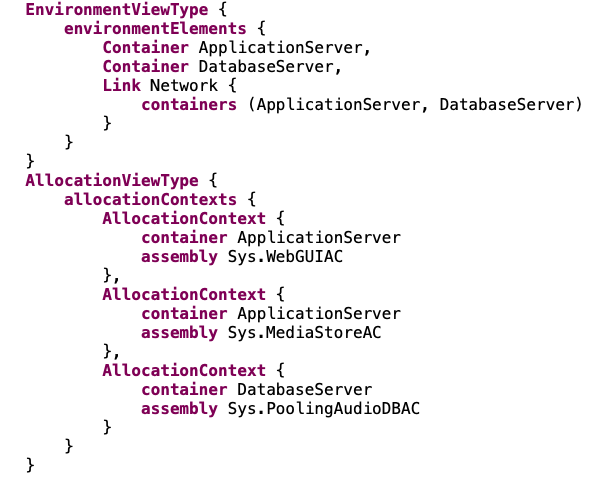
\includegraphics[height=40mm]{figures/xtext.png}
    \begin{itemize}
        \item Ergebnis: \texttt{mediastore.simplepalladio}
    \end{itemize}
\end{frame}

\begin{frame}{Probleme beim Entwurf der textuellen Syntax}
	\begin{enumerate}
		\item Problem: Import von Subpackages konnte nicht aufgelöst werden
		\begin{itemize}
            \item Lösung: Verwendung von alternativer Importschreibweise anstatt Ns URI
            \item \texttt{import "platform:/resource/SimplePalladio/.../*.ecore\#//..."}
        \end{itemize}
        \item Probleme: Proxy-Ausflösung zwischen XText Dateien
		\begin{itemize}
            \item erster Ansatz: für jeden ViewType eine XText Grammatik
            \item Lösung: Grammatik als Weaving-Modell der verschiedenen Modelle in einer Datei
            \item \texttt{<datei>.simplepalladio}
        \end{itemize}
        \item Problem: zyklischen Abhängigkeiten zwischen Elementen von SystemIndependentViewType und AssemblyViewType
        \begin{itemize}
            \item Lösung: Entkopplung des Zyklus durch Aufspaltung des SystemIndependentViewTypes und des AssemblyViewTypes in zwei Regionen
        \end{itemize}
        \item Problem: automatische Validierung des XText $\Rightarrow$ OCL Constraints werden automatisch ausgewertet $\Rightarrow$ führte zu Fehlern, da OCL Constraints defekt waren
	\end{enumerate}
\end{frame}